The purpose of the floor plan in the application is to be used as a navigation guide for the user. The user should be able to make a customised route to different booths, The default route should be a route between all the booths that the user has subscribed to.
Ideally it should also be possible to subscribe/unsubscribe to each booth. The location of the user is detected when the user scans an \ac{nfc} tag, the \ac{nfc} tag are placed around the exhibition and at booths, to provide the user with easy location determination.

\section{MapView vs MapFragment}
Our initial thought on how to implement the floor plan on the phone was to use the service provided by Google Maps. We knew that it could implemented on the phone because we had previously seen it being used in other applications. What we did not know, was if we could override the standard Google Maps tiles with our own custom tile set of the floor plan. A tile is a single picture containing a piece of the map. Depending on the zoom level each tile contain a smaller piece of the actual map.\\
\begin{figure}[H]
\centering
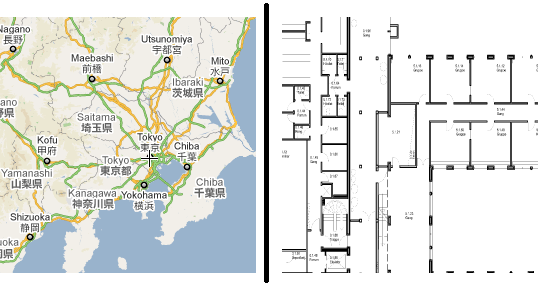
\includegraphics[width=0.8\textwidth]{img/tilessidebyside.png}
\caption{Google Maps tile and our custom tile \citep{googlemaptile}}
\label{fig:maptiles}
\end{figure}
We need to implement our own custom tile set because we want to show the floor plan of a building, instead of a map of the Earth. We read the documentation provided by Google Maps\citep{googlemapsapi}, and we found that it is not possible to override the standard tiles with your own tiles to the Android MapFragment. But this was possible when using the \ac{api} for JavaScript. We then thought of implementing the floor plan with a WebView which is basically a browser inside the application, and use JavaScript to create the map. With JavaScript it is possible to override the standard tile set with your own, but the performance on the phone was horrible so we scratched the idea. After some research we found a solution to our problem, we use a MapFragment and instead overriding the standard tile set we simply hide them, and only show our custom tile set of the floor plan.

\section{Mercator projection}
\label{sec:mercatorprojection}
We are set upon using the Google Maps \ac{api}, and maps shown with Google Maps is default done with the Mercator projection. Mercator projection is a way of displaying a sphere on a two dimensional map.
There are a lot of ways of projecting a sphere on a map, but one of the most successful is the Mercator projection. The Mercator projection is often chosen because of it navigational properties. One of the biggest navigational properties Mercator provides, is it's ability to represent lines of constant course as straight lines.\\
A Mercator projected map is illustrated by Figure \autoref{fig:mercatorexplain}. Let the globe be a spherical balloon, the balloon is blown up inside a cylinder, and sticks to the cylinders side as it is blown up. The three first pictures on Figure \autoref{fig:mercatorexplain} shows the balloon being blowing up, the last picture shows the cylinder being cut open and displayed as a two dimensional map.
\begin{figure}[H]
\centering
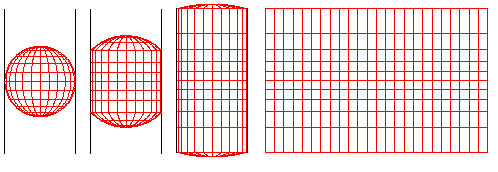
\includegraphics[width=0.8\textwidth]{img/mercatorexplain.png}
\caption{Explanation of Mercator projection \citep{mercatorexplain}}
\label{fig:mercatorexplain}
\end{figure}
The \autoref{fig:mercatorexplain} also shows how the top part(latitude) of the spherical balloon is stretched, for it to fit inside the cylinder. This is one of the disadvantages of the Mercator projection, the landmasses and continents are not scaled correctly.
\begin{figure}[H]
\centering
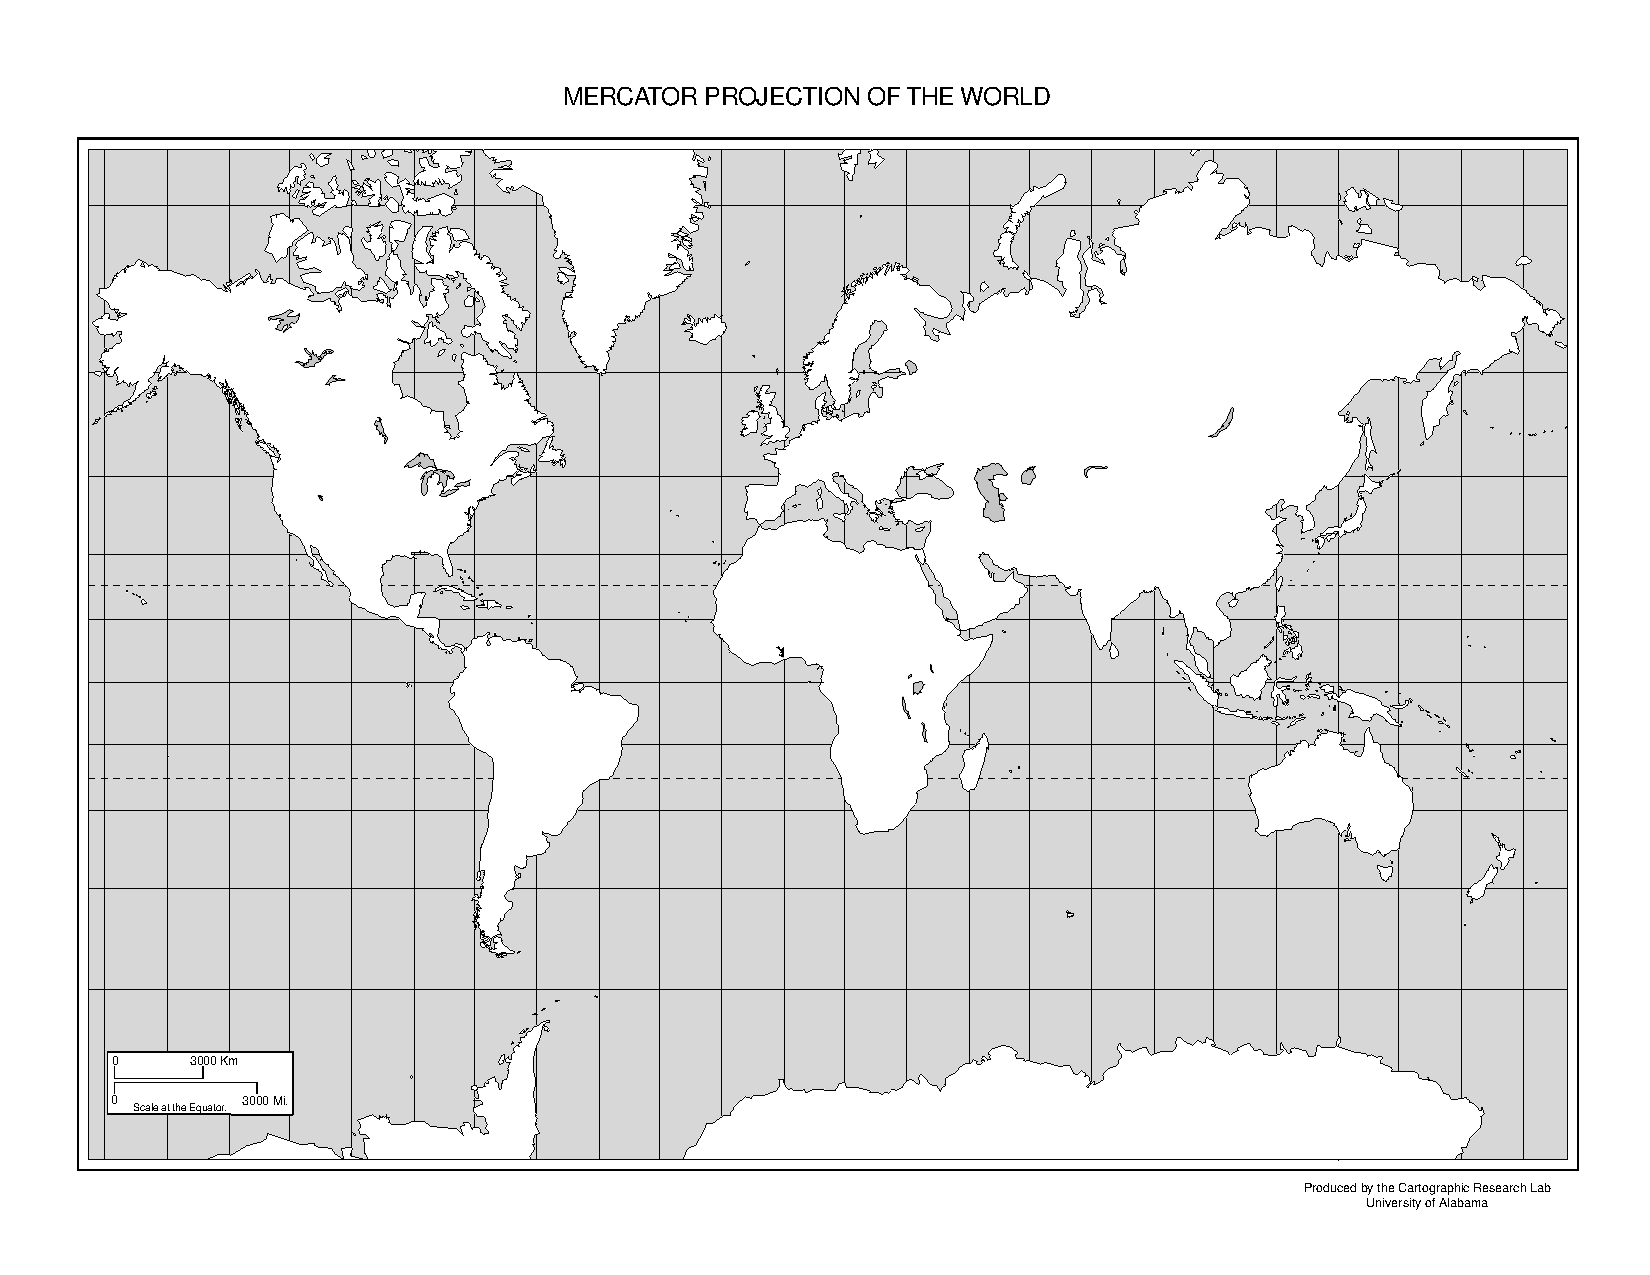
\includegraphics[width=0.7\textwidth]{img/mercatorworld.pdf}
\caption{The World - Mercator projection  \citep{mercatorworld}}
\label{fig:mercatorworld}
\end{figure} As seen on the \autoref{fig:mercatorworld} Greenland is almost the same size as Africa, but in reality Africa is 14 times bigger than Greenland.

\section{Google Maps}
We use the service provided by Google, called Google Maps, to present our floor plan. This service is normally used for displaying the Earth and for navigation. Google Maps uses the Mercator projection which is explained in a earlier \secref{sec:mercatorprojection}. Normally a map is distorted by the Mercator projection, but in our case this is not a problem, since our floor plan already is a plane. The Google Maps' \ac{api} is both available in JavaScript and Java(Android), although the Java \ac{api} has a few limitations.

\subsection*{Tiles}
The Google Maps \ac{api} allows the user to zoom on the floor plan, the floor plan is shown on \autoref{fig:cassiopeia}. Zooming on the floor plan allows us to present the floor plan in more detail. For this to work we need to split our original floor plan picture into small tiles, the tiles are always the size 256$x$256 pixels. As the zoom level increases the more tiles are needed to present the floor plan, so at zoom level 2 the floor plan will be rendered as  a 4$x$4 grid. At zoom level 3 a 8$x$8 grid, and so on. \autoref{fig:tilecoordinates} shows how the original picture is split into tiles at zoom level 3. Each zoom level has to be stored on either a server or locally.

\begin{figure}[H]
\centering
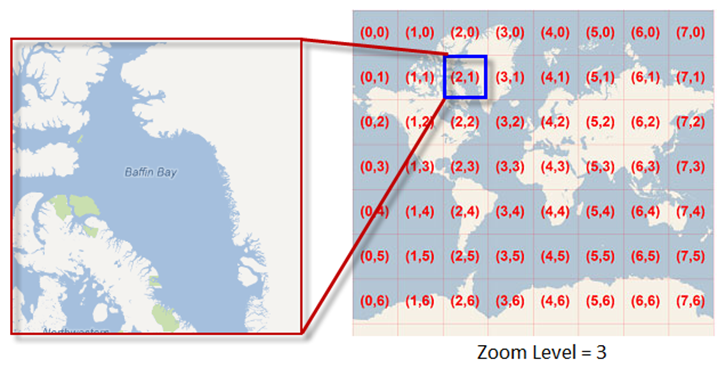
\includegraphics[width=0.7\textwidth]{img/tilecoordinates2.png}
\caption{Tile split example with zoom level 3 \citep{tilecoordinates}}
\label{fig:tilecoordinates}
\end{figure}

\subsection*{Map Elements}
The Google Maps \ac{api} also allows us to draw different shapes and elements onto the floor plan. In this section we will show and explain how these elements are created and used.

\subsubsection*{Markers}
Markers are used to identify locations on the floor plan. The marker's icon is customisable so it can be used to differentiate between the types of locations. Markers are also equipped with a info windows, which popup if the marker is pressed. The info windows is used to give a short description about the location. We use the markers the display the information about the booths and also the position of the user on the floor plan. An example on markers are the small info markers, as seen on \autoref{fig:markerandboothexample}. 
\begin{figure}[H]
\centering
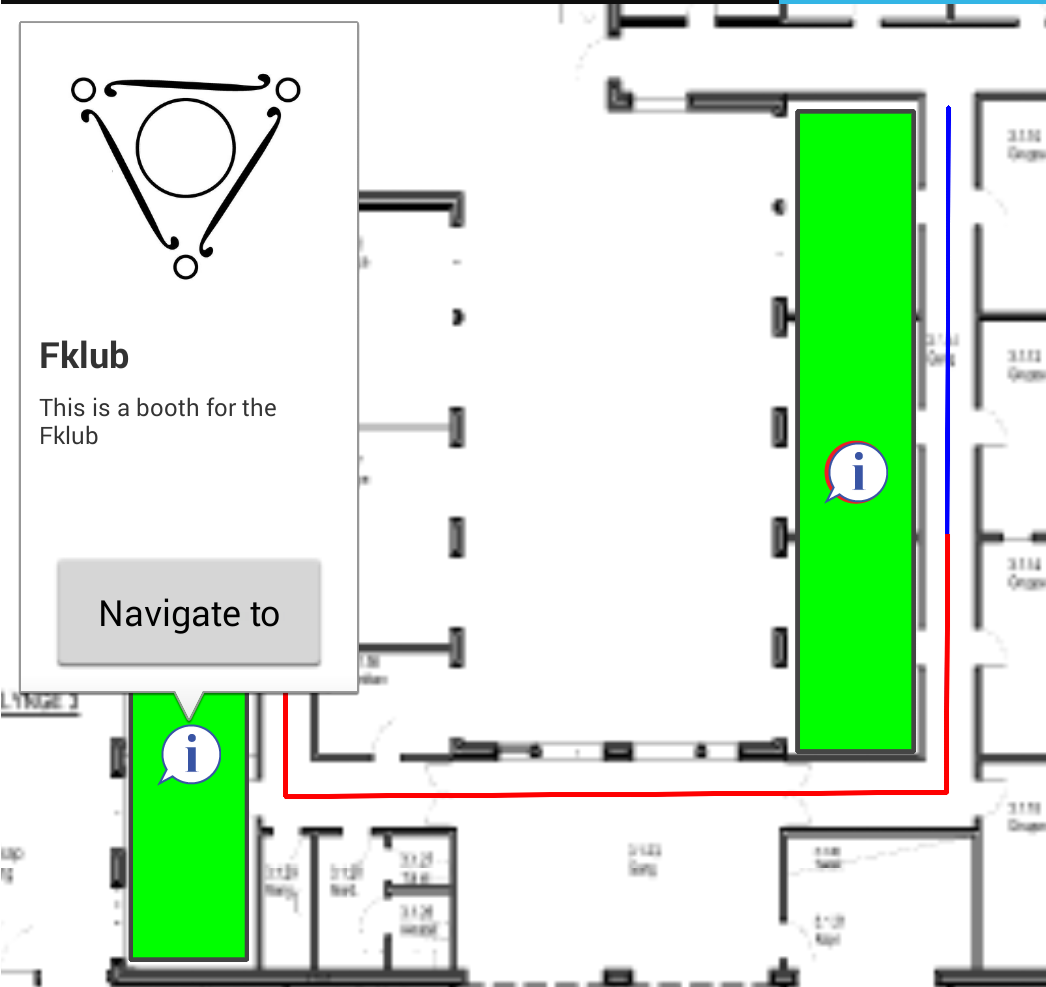
\includegraphics[width=0.7\textwidth]{img/markerandbooth.png}
\caption{Marker and booth example}
\label{fig:markerandboothexample}
\end{figure}
\todo{Show how they are drawn}

\subsubsection*{Polylines}
Polylines presents a set a of connected line segments on the floor plan. The Polyline object consists of a set of latitude and longitude coordinates, and creates a connected line between all the coordinates in a ordered sequence. The polyline's colour can also be customised to differentiate between other polylines. We use the polyline to show the walk path on the floor plan, and also showing the route to different booths from the user's location. \autoref{fig:polylineexample} shows an example of a polyline, the array that defines the polyline on \autoref{fig:polylineexample} would look like this \lstinline|{NodeA, NodeB, NodeC, NodeB, NodeD}|.  
\begin{figure}[H]
\centering
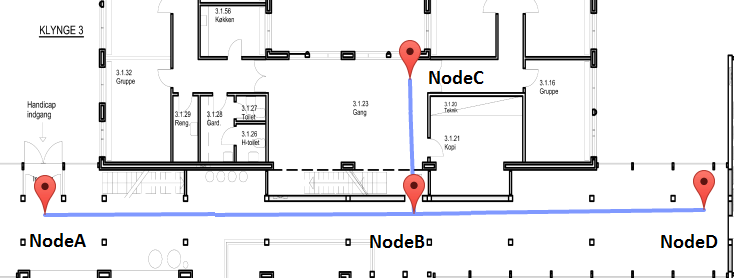
\includegraphics[width=0.9\textwidth]{img/polylineExample.png}
\caption{Polyline example}
\label{fig:polylineexample}
\end{figure}
\todo{Show how they are drawn}

\subsubsection*{Polygons}
Polygons are similar to polylines in that they consist of a series of latitude and longitude coordinates. But instead it being a line segment that is open, the polygons are designed to be a closed region. The polygon's interior is also filled with a colour. With makes it perfect for showing booths on our floor plan.
On \autoref{fig:markerandboothexample} the green shape shows a polygon, The green shape represents a booth.
\todo{Show how they are drawn}

\section{Implementation of Floor Plan}
In this section we will explain how we implemented our map of the floor plan using Google Maps. Implementing the default map on an Android phone is actually simple. All that is needed is to implement a fragment called "MapFragment" onto an activity.

\subsection*{Tile Provider}
With the implemented MapFragment it is possible to display an overlay with your own custom tile set. This is done by providing the MapFragment with a UrlTileProvider\citep{tilecoordinates}. This class has a method called \lstinline|getTileUrl()| that specifies how to get each tile. The method will be automatically called by the MapFragment every time the user moves into an region where tiles still hasn't been loaded. The parameters for \lstinline|getTileUrl()| is the tile's x,y coordinate, as seen on \autoref{fig:tilecoordinates}, and the current zoom level.\\
Our tile set is stored on the URL "figz.dk/dl/FloorPlan/". A tile is uniquely identified with the URL "figz.dk/dl/FloorPlan/zoom-level/x/y.png". We have created tiles from zoom level 2 to 6, meaning that we have $4^2+8^2+16^2+32^2+64^2 = 5456$ tiles. We could easily have created more zoom-levels and thereby tiles, but our example floor plan does not require much detail, and it would be confusing if the user could zoom closer. When our custom tile set is created and shown, we can simply hide the standard Google Maps Earth tile set. This is done simply to avoid loading unnecessary data.

\subsection*{Loading the Walk Path}
With the MapFragment implemented and the tiles loaded, we can draw the walk path of the exhibition. The walk path has previously been made and uploaded to the database by our web tool, which will be explained in the following \secref{sec:websiteimplementation}. When the walk path has been created, we load the nodes and edges from the database. With the nodes and edges we create a graph object, and from this undirected graph we create a polyline.\\ 
The polyline has a special structure, each of its elements is a latitude and longitude coordinate and between each coordinate pair, a line segment is drawn. The polyline's coordinates are defined as if you were to draw a walk path on a map, but you could never let go or lift the pencil from the paper, as seen on\autoref{fig:polylineexample}. Meaning that in order to create the polyline we might need to define an edge more than once. \autoref{lst:makePolyLine} shows the method that we use to make our walk path, and the shortest path polyline, from the undirected graph.
\begin{lstlisting}[language=java, label=lst:makePolyLine, caption=makePolyLine]
public void makePolyLine(){
        this.polylinePath = new ArrayList<Node>();
        for(Edge edge : this.getEdges()){
            int indexNodeA = this.polylinePath.indexOf(edge.getNodeA());
            int indexNodeB = this.polylinePath.indexOf(edge.getNodeB());
            
            if(indexNodeB != -1){
               this.polylinePath.add(indexNodeB + 1, edge.getNodeA());
               this.polylinePath.add(this.polylinePath.indexOf(edge.getNodeA())+1, edge.getNodeB());
            }
            else if(indexNodeA != -1 ){
               this.polylinePath.add(indexNodeA + 1, edge.getNodeB());
               this.polylinePath.add(this.polylinePath.indexOf(edge.getNodeB())+1, edge.getNodeA());
            }
            else{
               this.polylinePath.add(edge.getNodeA());
               this.polylinePath.add(edge.getNodeB());
            }
        }

        ArrayList<LatLng> polyLine = new ArrayList<LatLng>();
        for(Node n : this.polylinePath){
            polyLine.add(n.getPosition());
        }
    }
\end{lstlisting}
\begin{description}
\item[Line 2] Start by creating a local array called  \lstinline|polyLinePath|, which consists of nodes.
\item[Line 3-5] For each edge in our undirected graph, get the index of Node A and B in the newly created array \lstinline|polyLinePath|.
\item[Lines 7-10] If Node B already exists in the \lstinline|polyLinePath| insert the two nodes in the following order (...,NodeB, NodeA, NodeB, ...)
\item[Lines 11-14] If Node A already exists in the \lstinline|polyLinePath| insert the two nodes in the following order (...,NodeA, NodeB, NodeA, ...)
\item[Lines 15-18] Else just add the two nodes to the array, this will only be done once.
\item[Line 21-24] Now that the loop is done, simply add every node's latitude and longitude to an array called \lstinline|polyLinePath|, which is the result of the function. 
\end{description}

\subsection*{Route and Limitations}
Now that we can present the graph on the map, with the polyline walk path. We want to find the shortest path between two nodes, for this we use the Dijkstra's shortest path algorithm. We will not go into detail how this is implemented since it is fairly simple. With our graph object we can calculate the shortest path. The weights of the edges is simply the distance between two nodes, and from this we can find the shortest route between the two nodes, source and target.\\ 
A user can set his target/destination by pressing on a booth's marker and press the button "Navigate to" in the info window, a red polyline will appear on the floor plan showing the shortest route, but only if the user has a known position.\\
If a \ac{nfc} tag is scanned and the tag has a node id stored on it, the application will automatically show the floor plan, zoom onto the location of the node displaying a red dot, and updating the user's position/source. The shortest path(red polyline) between the target and the user's new position is calculated from the undirected graph. The result will me made into a polyline with the method  \autoref{lst:makePolyLine} and drawn onto the floor plan, like the walk path. This is done every time the user scans a \ac{nfc} and changes his position.\\
If the scanned node is connected to a booth, meaning the node is a booth's entry point, then the red dot's position will be portrayed on the booth instead on the walk path.\\ 
At the moment the floor plan implementation can only show a route between two nodes, It is not possible to show a route between multiple destinations or nodes. Also it is not possible to unsubscribe from a booth, directly from the floor plan.







	
